\documentclass[border=4pt]{standalone}
\usepackage{tikz}
\usetikzlibrary{positioning, arrows.meta, shapes.geometric, calc, fit, backgrounds, shadows}
\usepackage{amsmath,amssymb}

\begin{document}
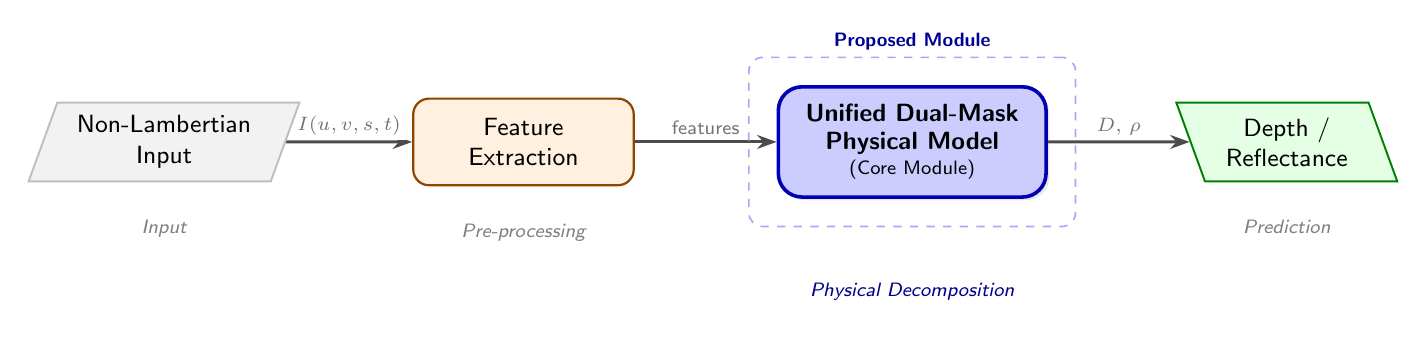
\begin{tikzpicture}[
  % ---- Style definitions ----
  input/.style={
    draw, trapezium, trapezium left angle=70, trapezium right angle=110,
    minimum width=2.4cm, minimum height=1.0cm,
    fill=gray!10, draw=gray!50, line width=0.7pt,
    align=center, font=\sffamily\small
  },
  proc/.style={
    draw, rounded corners=2mm, minimum width=2.8cm, minimum height=1.1cm,
    fill=orange!12, draw=orange!55!black, line width=0.8pt,
    align=center, font=\sffamily\small
  },
  innov/.style={
    draw, rounded corners=3mm, minimum width=3.4cm, minimum height=1.4cm,
    fill=blue!20, draw=blue!70!black, line width=1.3pt,
    align=center, font=\sffamily\small\bfseries,
    drop shadow={shadow xshift=1.2pt, shadow yshift=-1.2pt, opacity=0.18}
  },
  output/.style={
    draw, trapezium, trapezium left angle=110, trapezium right angle=70,
    minimum width=2.4cm, minimum height=1.0cm,
    fill=green!10, draw=green!50!black, line width=0.7pt,
    align=center, font=\sffamily\small
  },
  arr/.style={
    -{Stealth[length=7pt, width=5pt]}, line width=1.1pt, color=black!70
  },
  lbl/.style={
    font=\sffamily\scriptsize, text=black!55, fill=white, inner sep=2pt
  },
  gbox/.style={
    draw=blue!35, dashed, rounded corners=5pt, inner sep=10pt, line width=0.6pt
  },
]

% ---- Nodes (left to right) ----
\node[input] (m1) {Non-Lambertian\\Input};

\node[proc, right=1.6cm of m1] (m2) {Feature\\Extraction};

\node[innov, right=1.8cm of m2] (m3) {Unified Dual-Mask\\[-1pt]Physical Model\\[-2pt]\scriptsize\mdseries (Core Module)};

\node[output, right=1.8cm of m3] (m4) {Depth /\\Reflectance};

% ---- Main flow arrows (on background layer) ----
\begin{pgfonlayer}{background}
  \draw[arr] (m1) -- node[lbl, above] {$I(u,v,s,t)$} (m2);
  \draw[arr] (m2) -- node[lbl, above] {features} (m3);
  \draw[arr] (m3) -- node[lbl, above] {$D,\,\rho$} (m4);
\end{pgfonlayer}

% ---- Decorative grouping around the core innovation ----
\begin{scope}[on background layer]
  \node[gbox, fit=(m3),
        label={[font=\sffamily\scriptsize\bfseries, text=blue!60!black,
                fill=white, inner sep=2pt]above:Proposed Module}] {};
\end{scope}

% ---- Stage labels under the pipeline ----
\node[font=\sffamily\scriptsize\itshape, text=black!50,
      below=0.35cm of m1] {Input};
\node[font=\sffamily\scriptsize\itshape, text=black!50,
      below=0.35cm of m2] {Pre-processing};
\node[font=\sffamily\scriptsize\itshape, text=blue!55!black,
      below=0.95cm of m3] {Physical Decomposition};
\node[font=\sffamily\scriptsize\itshape, text=black!50,
      below=0.35cm of m4] {Prediction};

\end{tikzpicture}
\end{document}